\documentclass[10pt, pscyr, nonums]{hedlabwork}
\usepackage[russian]{babel}
\usepackage{hedmaths}
\usepackage{graphicx}
\graphicspath{{images/}, {plots/}}

\newgeometry{top=1.5cm, bottom=1.5cm, left=1cm, right=1cm}

\student{Слоква В. И., Ф-469}
\date{02.10.2013}
\labnum{605}
\labname{Определение ширины запрещенной зоны в кристалле диэлектрика}

\begin{document}
    \makeheader

    \emph{Цель работы:} изучение закономерностей поглощения света кристаллами с
    точки зрения зонной теории. Определение границы основного поглощения и
    ширины запрещенной зоны кристалла титаната бария.
    
    \emph{Используемые при расчетах формулы:}
    \( \tau = (J - J_T)/(J_0 - J_T); \ \Delta E = hc/\lambda_0 \).

    \begin{figure}[h!]
        \center
        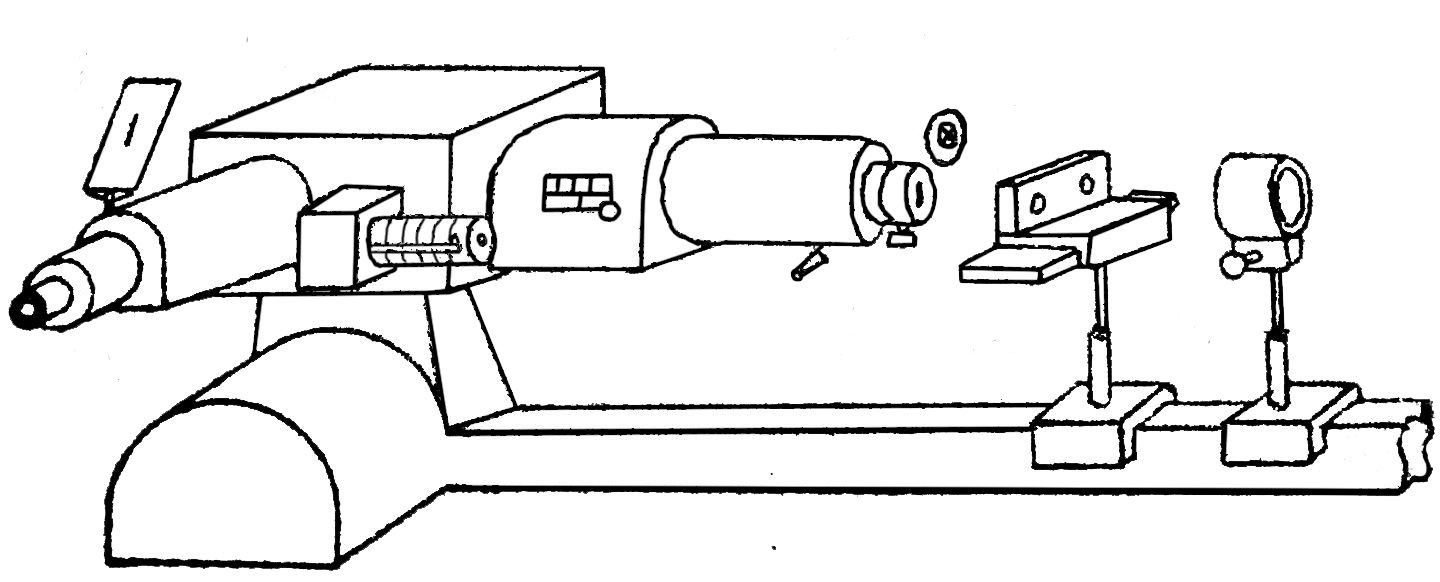
\includegraphics[width=.5\textwidth]{appearance} \\
        \parbox{.5\textwidth}{\caption{Внешний вид установки}}
    \end{figure}
    
    \begin{table}[h!]
        \center \caption{Однократно измеряемые величины и постоянные}
        \begin{tabular}{|*{8}{C{.1}|}} \hline
            \( \phi^* \),~град & \( \phi_{585} \),~град &
                \( \Delta\phi \),~град & \( \lambda_0 \),~нм &
                \( \Delta E \),~Дж & \( \Delta E \),~эВ &
                \( c \),~м/с & \( \hbar \),~Дж\( \cdot \)с \\ \hline
            2504 & 2500 & 4 & 411,5 & 4,83 \( \cdot 10^{-19} \) & 3 & \( 3 \cdot 10^8 \) &
                \( 1,\!05 \cdot 10^{-34} \) \\ \hline
        \end{tabular}
    \end{table}
    
    \begin{table}[h!]
        \center \caption{Многократно измеряемые величины}
        \begin{tabular}{|*{8}{C{.1}|}} \hline
            \multicolumn{2}{|c|}{Отсчет по} &
                Длина &
                \multicolumn{4}{c|}{Интенсивность света, прошедшего через} &
                Прозрач- \\ \cline{4-7}
            \multicolumn{2}{|c|}{монохроматору, град} &
                волны, нм &
                \multicolumn{2}{c|}{кристалл} &
                \multicolumn{2}{c|}{окно} &
                ность, \% \\ \hline
            \( \phi' \) & \( \phi \) & \( \lambda \) &
                \( J \) & \( J - J_T \) &
                \( J_0 \) & \( J_0 - J_T \) &
                \( \tau \) \\ \hline
            2120 & 2124 & 518   & 3    & 2,98 & 10,30 & 10,28 & 28,99 \\ \hline
            2020 & 2024 & 505   & 2,87 & 2,85 & 9,70  & 9,68  & 29,44 \\ \hline
            1920 & 1924 & 495   & 2,48 & 2,46 & 8,20  & 8,18  & 30,07 \\ \hline
            1820 & 1824 & 483   & 2,10 & 2,08 & 6,90  & 6,88  & 30,23 \\ \hline
            1720 & 1724 & 472   & 1,72 & 1,70 & 5,65  & 5,63  & 30,20 \\ \hline
            1620 & 1624 & 465   & 1,40 & 1,38 & 4,70  & 4,68  & 29,49 \\ \hline
            1520 & 1524 & 447   & 1,12 & 1,10 & 3,70  & 3,68  & 29,89 \\ \hline
            1420 & 1424 & 440   & 0,88 & 0,86 & 2,92  & 2,90  & 29,66 \\ \hline
            1320 & 1324 & 432   & 0,63 & 0,61 & 2,40  & 2,38  & 25,63 \\ \hline
            1220 & 1224 & 427   & 0,45 & 0,43 & 2,11  & 2,09  & 20,57 \\ \hline
            1120 & 1124 & 422   & 0,33 & 0,31 & 1,65  & 1,63  & 19,02 \\ \hline
            1020 & 1024 & 420   & 0,21 & 0,19 & 1,36  & 1,34  & 14,18 \\ \hline
            920  & 924  & 416   & 0,13 & 0,11 & 1,02  & 1,00  & 11,00 \\ \hline
            820  & 824  & 414,3 & 0,08 & 0,06 & 0,82  & 0,80  & 7,50  \\ \hline
            720  & 724  & 413,2 & 0,05 & 0,03 & 0,60  & 0,58  & 5,17  \\ \hline
            620  & 624  & 412,8 & 0,04 & 0,02 & 0,45  & 0,43  & 4,65  \\ \hline
            520  & 524  & 412,6 & 0,03 & 0,01 & 0,30  & 0,28  & 3,57  \\ \hline
        \end{tabular}
    \end{table}
    
    \pagebreak
    
    \subsection{Подсчет погрешности и окончательные результаты}
    \center
    \rule{.95\textwidth}{.5pt} \\ \rule{.95\textwidth}{.5pt}
    \rule{.95\textwidth}{.5pt} \\ \rule{.95\textwidth}{.5pt}
    \rule{.95\textwidth}{.5pt} \\ \rule{.95\textwidth}{.5pt}
    \rule{.95\textwidth}{.5pt} \\ \rule{.95\textwidth}{.5pt}
    \rule{.95\textwidth}{.5pt} \\ \rule{.95\textwidth}{.5pt} \\
    \vspace*{2em}
    
    \emph{Вывод:} \rule{.885\textwidth}{.5pt}
    \rule{.95\textwidth}{.5pt} \\ \rule{.95\textwidth}{.5pt}
    \rule{.95\textwidth}{.5pt}
\end{document}
